\begin{figure}[htbp]
\centering
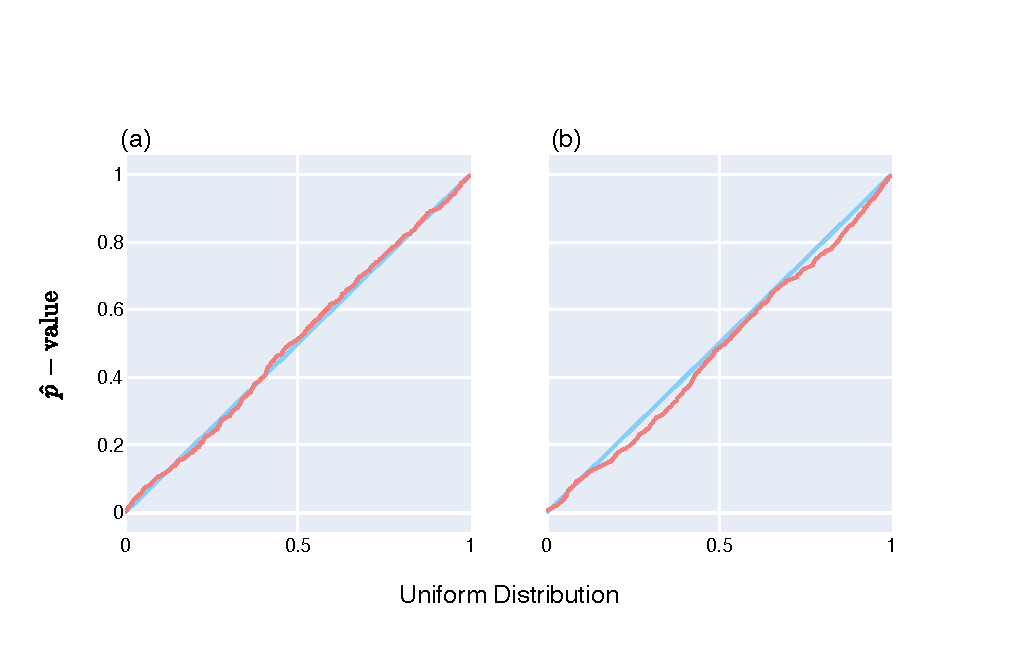
\includegraphics[width=\textwidth]{figures/plots/synthetic/adj-temp_eop/High JSD, High Entropy.pdf}
\caption{\textbf{Both equivalence of process tests were consistent with theoretical approximations.} The Quantile-Quantile plots compare the distribution of $\hat p-$values to the uniform distribution. As the data points (shown as the pink line) fall very close to the diagonal, this demonstrates that the distribution of $\hat p-$values is almost indistinguishable from the uniform distribution. (a) $\hat p-$values from temporal equivalence of process, (b) $\hat p-$values from adjacent equivalence of process. Each data set contains 1,000 synthetic stationary alignments. This result is shown for alignments of length 300 generated by the High JSD, High Entropy seed, however, the result was the same for all seeds and all lengths, shown in the appendix, see figure \ref{fig:synthetic/adj_eop/all_seeds} and \ref{fig:synthetic/temp_eop/all_seeds}.}
\label{fig:synthetic/adj-temp_eop/HighJSDHighEntropy}
\end{figure}